\subsection{Heatmaps}
A Markov transition matrix, which captures the probabilities of transitioning from one state to another in a Markov chain, can be effectively visualized as a heatmap to reveal underlying patterns and structures in the data. Each entry in the matrix corresponds to the probability of moving from a given state to another, and when represented as a heatmap, these probabilities are depicted as varying intensities of color. This visualization allows for the immediate identification of prominent transitions (high probability values), which appear as brighter or more intense areas, while less likely transitions are represented by darker or subdued tones. \cite{genc2019optimal} 


\begin{figure}[H]
    \centering
    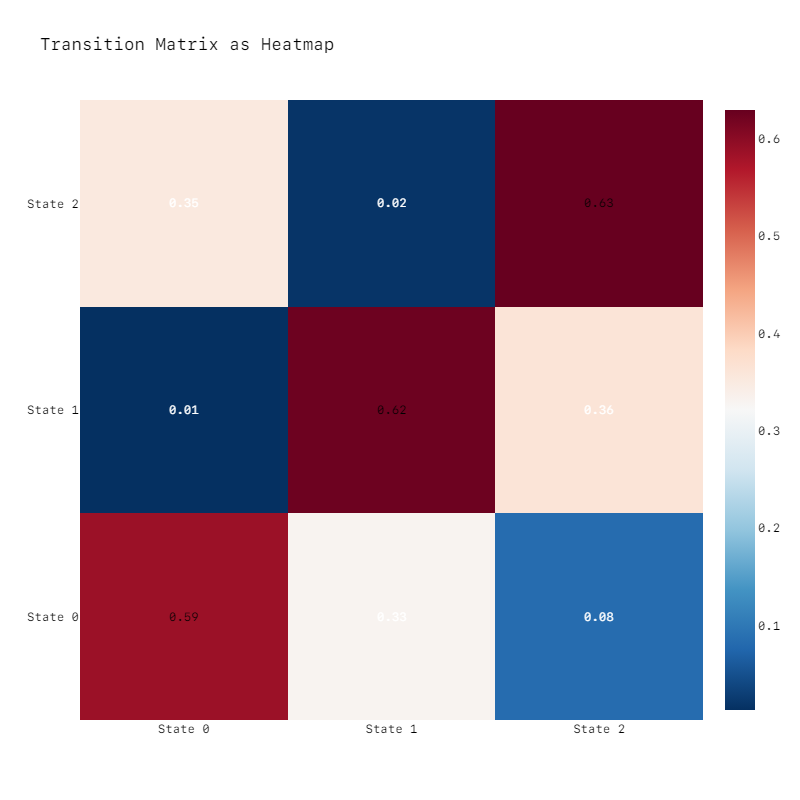
\includegraphics[width=0.5\textwidth]{images/heatmap.png}
    \caption{Heatmap of a Markov transition matrix}
    \label{fig:heatmap}
\end{figure}

\subsection{Directed Acyclic Graphs}
A Bayesian network, which represents a set of variables and their conditional dependencies via a probabilistic graphical model, can be effectively visualized as a Directed Acyclic Graph (DAG). In this representation, each node in the DAG corresponds to a variable, and directed edges between nodes signify the conditional dependencies, where an edge from node A to node B indicates that B is conditionally dependent on A. The acyclic nature of the graph ensures that there are no feedback loops, thereby maintaining the probabilistic consistency of the model. 


\begin{figure}[H]
    \centering
    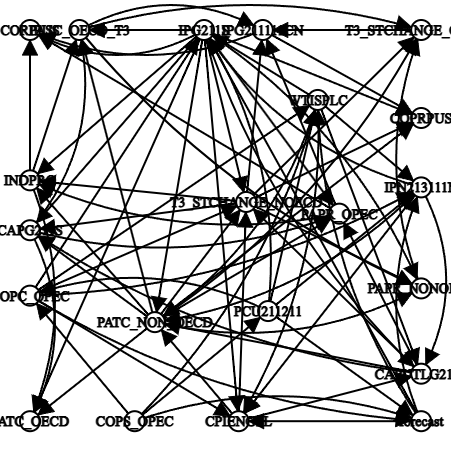
\includegraphics[width=0.5\textwidth]{images/graph.png}
    \caption{Heatmap of a Markov transition matrix}
    \label{fig:heatmap}
\end{figure}

